Antes de demonstrar os comparativos entre os gráficos e avaliar qual dos
algoritmos possuiu melhor desempenho, vamos basear a questão do desempenho
pela quantidade de \textit{page faults} reportados pela execução.
Como não é possível obter métricas reais do tempo de execução da escrita e
leitura do disco, o número de páginas não encontradas na memória será o
norteador.
A justificativa vem do motivo de que: uma vez que uma página não é encontrada
na memória é necessário acessar o disco para carregar as informações daquela
página.
Além disso, quando um \textit{pag fault} é reportado, e o programa já faz uso
de toda a memória disponível para sua própria execução, são necessárias duas
operações: A possível escrita de uma \textit{dirty page} no disco e a leitura
da página solicitada.
Portanto, o uso da quantidade de paginas não encontradas na memória possui uma
forte justificativa para ser utilizada como métrica nesse ambiente simulado
que fora apresentado por este trabalho.


\subsection{Algoritmo customizado}
Nessa análise, foi executado todas as combinações disponíveis entre
\textit{Tamanho da Página}, \textit{Memória Disponível} e
\textit{Arquivo de Entrada}. Após obter os resultados, para cada valor
de \textit{Memória disponível}, calculou-se a média da quantidade de 
\textit{page faults} entre todos os pares de \textit{Tamanho da página}
e \textit{Arquivo de entrada}.
Ou seja, um ponto no gráfico da Figura \ref{fig:grafico1} corresponde a um valor fixo
do \textit{Algoritmo} e da \textit{Memoria Disponível} em contraste com
a média das execuções que variaram o valor dos outros dois argumentos.

\begin{figure}[h]
	\begin{center}
		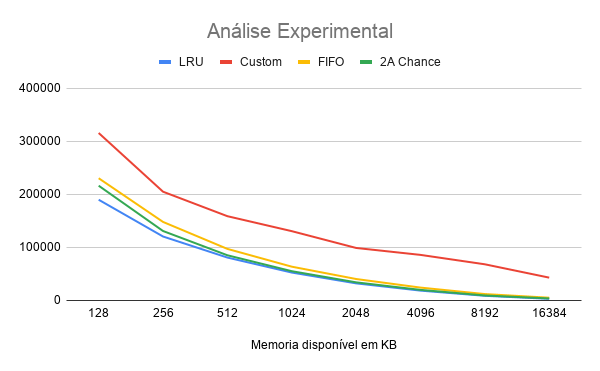
\includegraphics[scale=0.7]{Figuras/img1.png}
	\end{center}
	\caption{\label{fig:grafico1} }
\end{figure}

No gráfico da Figura \ref{fig:grafico1}, observamos que o algoritmo customizado
obteve uma quantidade de \textit{page faults} muito maior que os demais.
Podemos observar então, que esse tipo de hashing não é eficiente para essa aplicação
uma vez que muitos endereços possuem o conjunto dos bits menos significativos muito
próximos.
Possivelmente, uma abordagem melhor, seria criar tal hashing pelo bits mais
significativos, uma vez que valores de endereços com bits mais significativos
muito diferentes, identificam que tais endereços estão dispersos.
Entretanto, foi solicitado pelo trabalho um algoritmo de reposição ainda não
difundido, e o algoritmo que utiliza um tipo de hashing com os bits mais 
significativos é aplicado em hardware para a transição entre memória RAM e 
caches do processador.


\subsection{Tamanho de página constante e variação da memória disponível}
Para tal abordagem, mantivemos constantes o tamanho de cada página, em 4 Kilo
Bytes. Entretanto, variamos o tamanho da memória disponível entre o intervalo
de 128 a 1638 Kilo Bytes.
Além disso, como são 4 arquivos de entrada, também variamos tais arquivos, porém
realizamos uma análise da média de execução entre estes quatro arquivos.
A inclusão do algoritmo \texttt{custom} nessa análise, interferiria na qualidade
do gráfico, uma vez que os valore dos resultados do método customizado são muito
grandes.
Isso acarretaria numa aproximação entre as linhas dos outros três métodos de
reposição, fazendo com que eles ficassem muito semelhantes a "olho nu".
Além disso, na especificação desse trabalho, solicitou-se esse comparativo apenas
para os \textit{FIFO}, \textit{LRU} e \textit{2A Chance}.
O gráfico dessa extração de dados está contido na Figura \ref{fig:grafico2}.

\begin{figure}[h]
	\begin{center}
		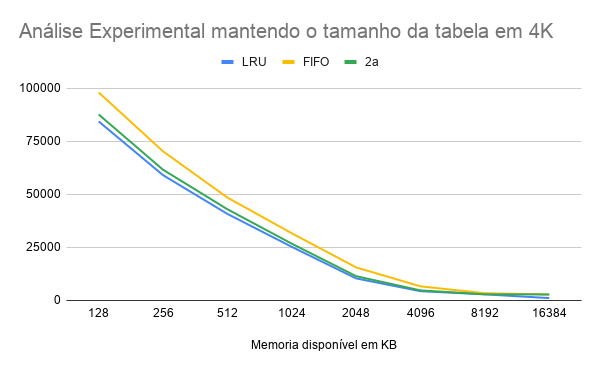
\includegraphics[scale=0.7]{Figuras/img2.png}
	\end{center}
	\caption{\label{fig:grafico2} }
\end{figure}

A análise visual, permite identificar uma aproximação de desempenho entre os métodos.
Porém é possível notar que \textit{FIFO} performou pior que os demais, uma vez que para
uma mesma quantidade de memória disponível e uma mesmo tamanho de página, esse método
possui um número maior de \textit{page faults}.
Porém, com o crescimento da quantidade de memória disponível, observou-se uma forte
aproximação do \textit{FIFO} com o método \textit{2A Chance} e há uma razão
por trás desse fato.
Ambos os algoritmos de reposição utilizam uma lista circular para apontar a próxima
pagina que será reposta no disco em caso de necessidade.
Entretanto, com diz o nome, \textit{2A Chance} aplica uma revalidação que dá a uma pagina
uma chance a mais de permanecer na lista.
Com uma memória disponível grande, a nova chance concedida às páginas não terá impacto
se comparado ao \textit{FIFO} tradicional.
Já o método \textit{LRU} possui um melhor desempenho que todos os algoritmos
independentemente do cenário, entretanto o à medida que a memória disponível cresce
o desempenho do \textit{LRU} também converge, juntamente com os outros dois métodos
de substituição de páginas.


\subsection{Variação do tamanho da página vs. Memória Constante}
Neste ultimo caso, apresentado na Figura \ref{fig:grafico3} mantivemos a quantidade
de memória constante em 512 Kilo Bytes e variamos o tamanho das páginas.
Assim como nos demais casos, das seções anteriores, os valore de \textit{page faults}
são referentes à media dentre os quatro arquivos de entrada fornecidos.
Comparando as Figura \ref{fig:grafico2} e \ref{fig:grafico3} o algoritmo
\textit{LRU} também possui
uma performance melhor do que os demais, sendo que \textit{2A Chance} tem 
comportamento semelhante, porém com um pequeno gap que a faz desse método menos
eficaz.


\begin{figure}[h]
	\begin{center}
		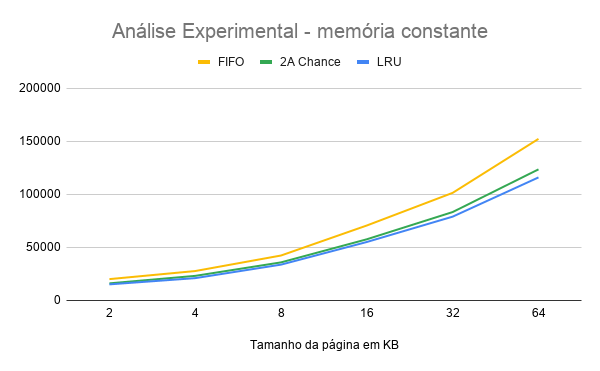
\includegraphics[scale=0.7]{Figuras/img3.png}
	\end{center}
	\caption{\label{fig:grafico3} }
\end{figure}

Na Figura \ref{fig:grafico3} também não incluímos o desempenho de \texttt{custom},
pois esse método se apresentou ineficaz e assim como na seção 4.1, a inclusão das
métricas desse gráfico atrapalharia a visualização das demais informações.
Outro fato que merece antenção é de que, em todos os gráficos observamos um aumento
na quantidade de \textit{page faults} à medida em que o tamanho da página aumenta.
Também há uma melhora de desempenho à medida em que a memória disponível aumenta.
O que demonstra uma dependência forte do desempenho dos algoritmos com o espaço
disponível.
Um possível algoritmo que conseguiria reduzir ou ter um impacto diferente destes
apresentados aqui, seria algum algoritmo preditivo, o qual alocaria as páginas
na memória baseado em fatores futuros, mas ainda assim haveria tal dependência.
